% Problem and Data -- handbook section 2.3 requires this coverage
% Motivation, task definition, dataset, and the exploratory findings that shape the method.
% Figures are read from ../results/eda/, which notebooks/eda.ipynb writes, so the slides
% always show the committed EDA output.

\section{Problem and Data}

%----------------------------------------------------------
\begin{frame}{Problem Formulation}
\begin{itemize}
    \item \textbf{Task:} semantic segmentation of urban street scenes, one prediction \emph{per pixel}.
    \item \textbf{Input:} an RGB frame $x \in \mathbb{R}^{3 \times H \times W}$.
    \item \textbf{Output:} per-pixel logits $z = f_\theta(x) \in \mathbb{R}^{19 \times H \times W}$;
          the prediction is $\hat{y}_{ij} = \arg\max_c z_{cij}$, so one $512 \times 1024$ frame
          carries $524{,}288$ predictions.
    \item \textbf{Research question:} with the data, the split and the protocol fixed, how much of
          the gap between a from-scratch model and a pretrained one comes from \emph{pretrained
          features}, and how much from architecture, loss or capacity?
    \item \textbf{Dataset:} Cityscapes fine annotations~\cite{cordts2016cityscapes}.
    \item \textbf{Main difficulty:} the classes span almost three orders of magnitude in pixel
          share, and the output must keep spatial resolution all the way through.
\end{itemize}
\end{frame}

%----------------------------------------------------------
\begin{frame}{Cityscapes}
\scriptsize
\begin{columns}[T]
\begin{column}{0.48\textwidth}
\begin{itemize}
    \item \textbf{Source:} recorded from a vehicle in 27 cities; per-pixel polygons drawn by
          expert annotators~\cite{cordts2016cityscapes}.
    \item \textbf{Size:} 5{,}000 fine frames at $1024 \times 2048$; 11\,GB images, 808\,MB labels.
    \item \textbf{Licence:} non-commercial research and education, account required.
\end{itemize}
\end{column}
\begin{column}{0.48\textwidth}
\begin{itemize}
    \item \textbf{Classes:} 34 label ids, \textbf{19 evaluated}; the rest map to an ignore label
          excluded from loss and metrics.
    \item \textbf{Unlabelled:} 11.8\% of pixels, of which 7.7\% is the bonnet and rectification border.
    \item \textbf{Bias:} daylight, fair weather, European cities, one camera.
\end{itemize}
\end{column}
\end{columns}

\begin{figure}
    \centering
    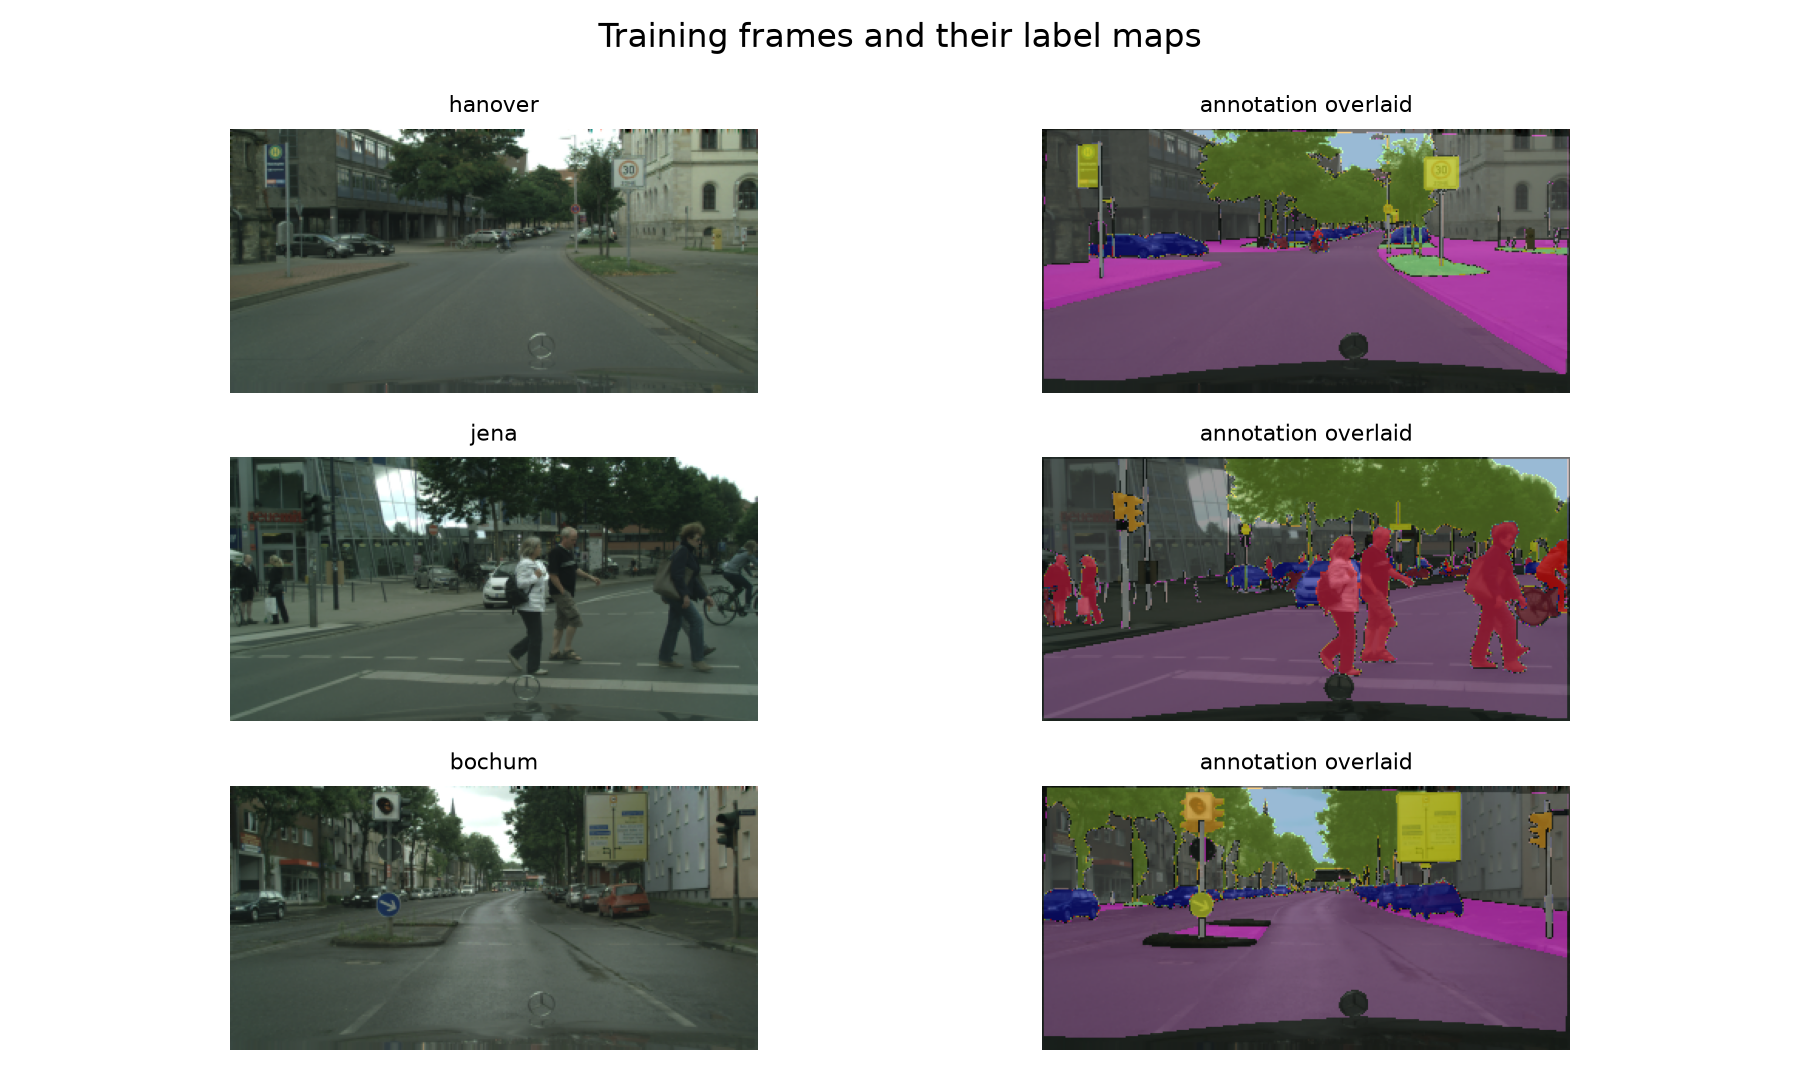
\includegraphics[width=0.38\textwidth]{../results/eda/samples.png}
\caption{Training frames and their label maps.}
\label{fig:samples}
\end{figure}
\end{frame}

%----------------------------------------------------------
\begin{frame}{Pixel Distribution Decides the Metric}
\begin{columns}[c]
\begin{column}{0.58\textwidth}
\begin{figure}
    \centering
    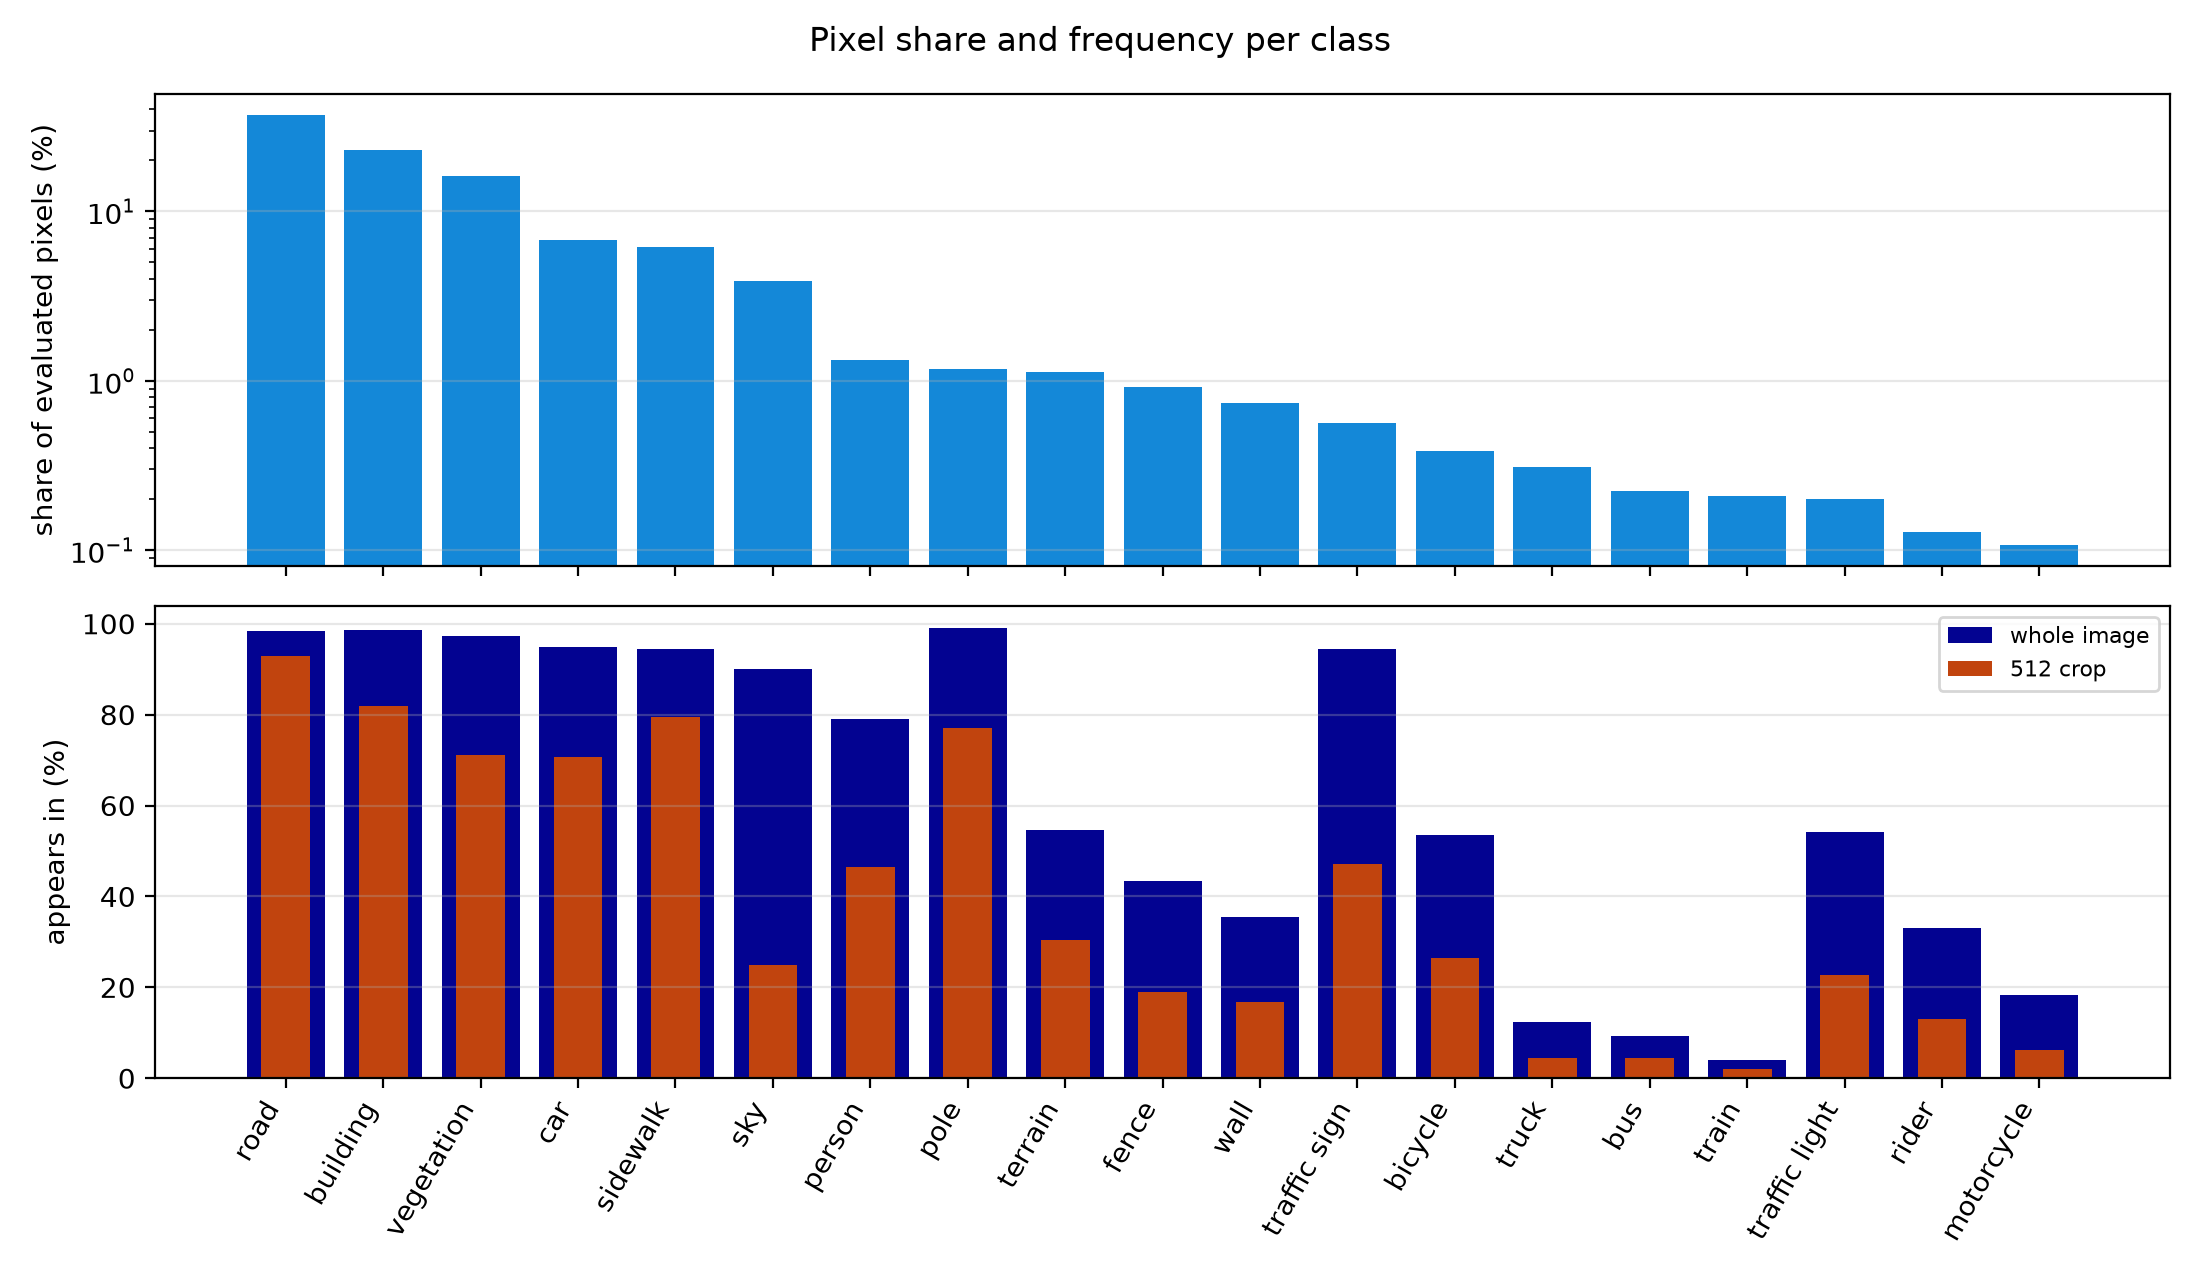
\includegraphics[width=\textwidth]{../results/eda/class_distribution.png}
\caption{Pixel share and frequency per class.}
\label{fig:class-distribution}
\end{figure}
\end{column}
\begin{column}{0.40\textwidth}
\small
\begin{itemize}
    \item \textbf{Three classes dominate:} road, building and vegetation cover \textbf{75.8\%} of
          evaluated pixels.
    \item Predicting \emph{only} those three already reaches about \textbf{0.76 pixel accuracy}.
    \item \textbf{So mIoU is primary} and pixel accuracy decides nothing: mIoU averages over
          classes, so the other sixteen cannot be hidden.
    \item Per-class IoU is always reported beside the mean.
\end{itemize}
\end{column}
\end{columns}
\end{frame}

%----------------------------------------------------------
\begin{frame}{Two Kinds of Scarcity, One Remedy Will Not Fix Both}
\small
\begin{table}
\centering
\caption{Two kinds of scarcity.}
\label{tab:scarcity}
\begin{tabular}{llrrrr}
\toprule
& \textbf{Class} & \textbf{Pixels} & \textbf{Images} & \textbf{Area when present} & \textbf{Crops} \\
\midrule
\multirow{2}{*}{\textit{Thin}} & pole         & 1.17\% & 99\% & 0.83\% & 77\% \\
                               & traffic sign & 0.56\% & 94\% & 0.31\% & 47\% \\
\midrule
\multirow{2}{*}{\textit{Rare but large}} & train & 0.21\% & \textbf{4\%} & 0.91\% & 2\% \\
                                         & bus   & 0.22\% & \textbf{9\%} & 0.66\% & 4\% \\
\bottomrule
\end{tabular}
\end{table}

\begin{itemize}
    \item \textbf{Thin classes} are never short of examples: poles appear in 99\% of images. They
          are lost to \emph{boundary imprecision}.
    \item \textbf{Rare-but-large classes} cover 3 to 4$\times$ their average share \emph{when
          present}, but are seldom seen at all.
    \item \textbf{Cropping sharpens the second:} trains fall from 4\% of images to 2\% of crops.
          Sky, present in 90\% of images, falls to 25\% of crops because it sits in a band.
    \item \textbf{A reweighted loss addresses the second, not the first}, which is why the
          ablation varies the loss.
\end{itemize}
\end{frame}

%----------------------------------------------------------
\begin{frame}{Splitting: the Unit Is the City}
\begin{columns}[T]
\begin{column}{0.46\textwidth}
\begin{table}
\centering
\small
\caption{Split sizes.}
\label{tab:splits}
\begin{tabular}{llrr}
\toprule
\textbf{Ours} & \textbf{Source} & \textbf{Cities} & \textbf{Images} \\
\midrule
Train & official train & 15 & 2{,}406 \\
Val   & official train & 3  &   569 \\
Test  & official val   & 3  &   500 \\
\bottomrule
\end{tabular}
\end{table}
\end{column}
\begin{column}{0.52\textwidth}
\small
\begin{itemize}
    \item \textbf{Why the city:} consecutive frames of one street share buildings, parked cars and
          road surface. Splitting by \emph{frame} would put near-duplicates on both sides.
    \item \textbf{Why not the official test:} its labels are withheld, so the official
          \emph{validation} partition serves as the test set.
    \item The three cities that \emph{select} the checkpoint therefore come out of train.
    \item \textbf{Leakage controls:} split committed as a file, not regenerated; normalization
          never from scored data; test read once, after selection.
\end{itemize}
\end{column}
\end{columns}
\end{frame}
